\documentclass[11pt,class=report,crop=false]{standalone}
\usepackage[screen]{../python}


\begin{document}


%====================================================================
\chapitre{Intégrale}
%====================================================================

\index{integrale@intégrale}

\objectifs{Nous allons étudier différentes techniques pour calculer des valeurs approchées d'intégrales.}


%%%%%%%%%%%%%%%%%%%%%%%%%%%%%%%%%%%%%%%%%%%%%%%%%%%%%%%%%%%%%%%%
%%%%%%%%%%%%%%%%%%%%%%%%%%%%%%%%%%%%%%%%%%%%%%%%%%%%%%%%%%%%%%%%

\begin{cours}[Primitive]
\index{primitive}
Soit $f : [a,b] \to \Rr$. Une \defi{primitive} de $f$ est une fonction dérivable 
$F : [a,b] \to \Rr$ tel que $F'(x) = f(x)$ pour tout $x\in [a,b]$.
Si on sait calculer une primitive alors on sait calculer l'intégrale de $f$ :
$$\int_a^b f(t) \;\dd t = F(b) - F(a).$$

Exemple : soit $f(x) = x^2$, une primitive de la fonction $f$ est la fonction $F$ définie par $F(x) = \frac13 x^3$, donc par exemple 
$\int_0^1 t^2\;\dd t = F(1)-F(0) = \frac13$.


\end{cours}

%%%%%%%%%%%%%%%%%%%%%%%%%%%%%%%%%%%%%%%%%%%%%%%%%%%%%%%%%%%%%%%%
% Activité 1
%%%%%%%%%%%%%%%%%%%%%%%%%%%%%%%%%%%%%%%%%%%%%%%%%%%%%%%%%%%%%%%%

\begin{activite}[Primitive]

\objectifs{Objectifs : vérifier expérimentalement si une fonction donnée $F$ est une primitive de $f$.}

\begin{enumerate}
  \item Programme une fonction \ci{verification_primitive(f,F,a,b,n,epsilon)}
  qui vérifie expérimentalement que $F$ est bien une de primitive de $f$ sur l'intervalle $[a,b]$ ($n$ est un entier donné, par exemple $n=10$ et $\epsilon$ une marge d'erreur, par exemple $\epsilon = 0.001$). 
  
  \emph{Méthode.} Vérifie que pour $n+1$ valeurs $x$ de $[a,b]$ on a
  $F'(x) \simeq f(x)$. Dans le détail :
  \begin{itemize}
    \item soit $x_k = a + k\frac{b-a}{n}$, $k=0,1,\ldots,n$ ;
    \item on calcule une valeur approchée de $F'(x_k)$ en utilisant la fonction \ci{derivee()} du chapitre \og{}Dérivée\fg{} ;
    \item on vérifie $F'(x_k) \simeq f(x_k)$ en testant si $\big| F'(x_k) - f(x_k) \big| \le \epsilon$ pour tout $k=0,\ldots,n$.
  \end{itemize}
  
   
  \item \'Ecris une fonction \ci{integrale_primitive(F,a,b)} qui calcule l'intégrale 
  d'une fonction $f$ connaissant une primitive $F$.
  
  \item \emph{Application.}
  \begin{enumerate}
    \item Calcule l'aire sous la parabole d'équation $y=x^2$ entre les droites verticales d'équation $(x=1)$ et $(x=2)$ et au-dessus de l'axe des abscisses.
    \item Même question avec l'aire sous le graphe de $f(x) = \sin(x)$ sur $[0,\pi]$.
  \end{enumerate}
  
\end{enumerate} 

\end{activite}

%%%%%%%%%%%%%%%%%%%%%%%%%%%%%%%%%%%%%%%%%%%%%%%%%%%%%%%%%%%%%%%%
%%%%%%%%%%%%%%%%%%%%%%%%%%%%%%%%%%%%%%%%%%%%%%%%%%%%%%%%%%%%%%%%

\begin{cours}[Calcul approché d'une intégrale]

% Avec du matériel venant du cours "Calcul formel"

Il n'est pas toujours possible de calculer une primitive pour une fonction $f : [a,b] \to \Rr$. On va déterminer des valeurs approchées de $\int_a^b f(t) \;\dd t$.

Les trois méthodes d'approximation que l'on va étudier sont toutes basées sur
le même principe : 
\begin{itemize}
  \item On divise l'intervalle $[a,b]$ en $n$ sous-intervalles en posant $x_k = a + k \frac{b-a}{n}$ pour $0\le k \le n$.
  Alors $x_0=a$ et $x_n = b$ et chaque sous-intervalle $[x_k,x_{k+1}]$ est de longueur constante $x_{k+1}-x_k= \frac{b-a}{n}$.
  
  
  
\myfigure{1}{
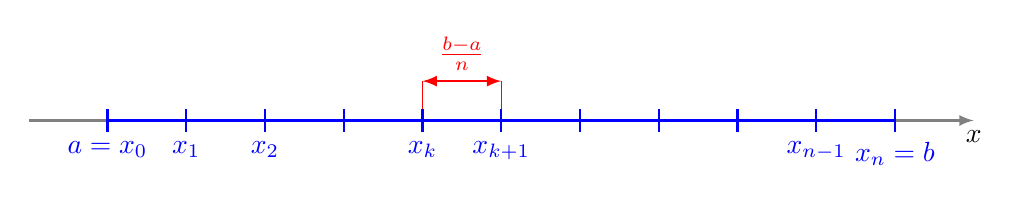
\begin{tikzpicture}[scale=1]


% Axes
     \draw[->,>=latex,thick, gray] (-1,0)--(11,0) node[below,black] {$x$};
 %    \draw[->,>=latex,thick, gray] (0,-0.05)--(0,1.5) node[right,black] {$y$};  


   \draw[very thick, blue] (0,0) -- (10,0);

  \draw [<->,>=latex,thick, red] (4,0.5) -- (5,0.5) node[midway, above] {$\frac{b-a}{n}$};
  \draw[thin,red] (4,0)--(4,0.5);
  \draw[thin,red] (5,0)--(5,0.5);

% Labels
  \foreach \x/\xtext in {0/{a=x_0}, 1/{x_1}, 2/{x_2},3/{},4/{x_k},5/{x_{k+1}},6/{},7/{},8/{},9/{x_{n-1}},10/{x_n=b}}
  \draw[thick, blue] (\x cm,4pt) -- (\x cm,-4pt) node[anchor=north] {$\xtext$};


  \node[below, inner sep=10pt] at (0.5,0) {\vphantom{$n=10$}};


\end{tikzpicture}

}  

  \item Sur chaque sous-intervalle $[x_k,x_{k+1}]$, on approche l'aire sous la courbe
  par l'aire d'une figure géométrique simple.
\end{itemize}

\begin{itemize}
  \item \textbf{Méthode des rectangles.} La \defi{méthode des rectangles (à gauche)} consiste à approcher l'aire sous la courbe par l'aire de rectangles. La hauteur de chaque rectangle est la valeur à gauche
de $f$ sur le sous-intervalle (voir les figures ci-dessous).
Pour un intervalle élémentaire, cela revient à approcher
$\int_{x_k}^{x_{k+1}} f(t)\;\dd t$ par $(x_{k+1}-x_k) f(x_k)$.

\myfigure{1}{
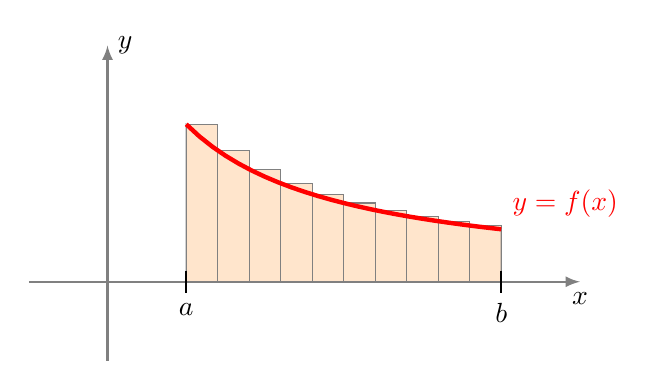
\begin{tikzpicture}[scale=2]

 
% Preparation pour rectangles

  \def\a{0}; \def\b{2};   \def\n{10}; 
  \pgfmathparse{\n - 1}
  \global\let\nmoins\pgfmathresult

\pgfmathparse{divide(\b-\a,\n)}
\let\dx\pgfmathresult

% Rectanglea gauche (au-dessus, en orange)

  \def\x{\a}
  \foreach \k in {0,1,...,\nmoins}{
  \pgfmathparse{\x}
  \global\let\xold\pgfmathresult

  \pgfmathparse{1/(1+\x)}
  \global\let\y\pgfmathresult

  \pgfmathparse{\x + \dx}
  \global\let\x\pgfmathresult

  %\filldraw[fill=green!20,draw=gray] (\xold,0) rectangle (\x,\y);
 \filldraw[fill=orange!20,draw=gray] (\xold,0) rectangle (\x,\y);
  }


% Axes
     \draw[->,>=latex,thick, gray] (-1,0)--(2.5,0) node[below,black] {$x$};
     \draw[->,>=latex,thick, gray] (-0.5,-0.5)--(-0.50,1.5) node[right,black] {$y$};  


% Graphe et aire
  \draw[gray] (0,0) -- plot[domain=-0:2] (\x,{1/(1+\x)}) -- (2,0) -- cycle;
  \draw[ultra thick, color=red,domain=0:2] plot (\x,{1/(1+\x)}) node[above right] {$y=f(x)$};

% Labels
  \foreach \x/\xtext in {0/a, 2/b}
  \draw[thick] (\x cm,2pt) -- (\x cm,-2pt) node[anchor=north] {$\xtext$};
%  \draw (1pt,1cm) -- (-1pt,1cm) node[anchor=east] {$1$};
%  \node[below, inner sep=10pt] at (0.5,0) {\vphantom{$n=10$}};

\end{tikzpicture}
\qquad
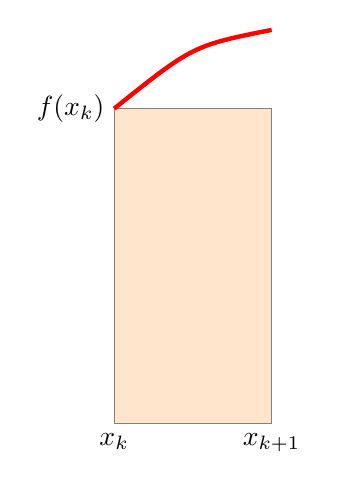
\begin{tikzpicture}[scale=2]

 

% Axes
%      \draw[->,>=latex,thick, gray] (-0.5,0)--(3,0) node[below,black] {$x$};
%      \draw[->,>=latex,thick, gray] (0,-0.05)--(0,3.5) node[right,black] {$y$};  
% 

% Graphe et aire


% Rectanglea gauche (en orange)
\filldraw[fill=orange!20,draw=gray] (1,0) rectangle (2,2);

  \draw[ultra thick, color=red] (1,2).. controls (1.5,2.4) ..  (2,2.5);

 \node[below] at (1,0) {$x_k$};
 \node[below] at (2,0) {$x_{k+1}$};
\node[left] at (1,2) {$f(x_k)$};


\end{tikzpicture}

} 
  
  \item \textbf{Méthode des trapèzes.}
 On approche l'aire sous la courbe d'un intervalle élémentaire, 
 par l'aire d'un trapèze.
 
 \myfigure{1}{
 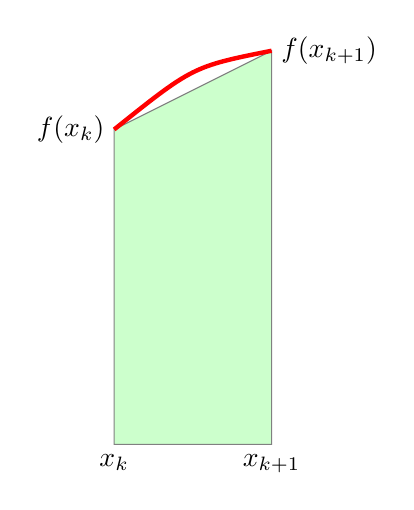
\begin{tikzpicture}[scale=2]



% Rectangle a droite (en vert)

\filldraw[fill=green!20,draw=gray] (1,0)--(1,2)--(2,2.5)--(2,0)--cycle;

  \draw[ultra thick, color=red] (1,2).. controls (1.5,2.4) ..  (2,2.5);

 \node[below] at (1,0) {$x_k$};
 \node[below] at (2,0) {$x_{k+1}$};
\node[left] at (1,2) {$f(x_k)$};
\node[right] at (2,2.5) {$f(x_{k+1})$};

\end{tikzpicture}

 } 
  
  \item \textbf{Méthode de Simpson.}
 On approche la courbe sur chaque intervalle élémentaire
par une branche de parabole. 
\myfigure{1}{
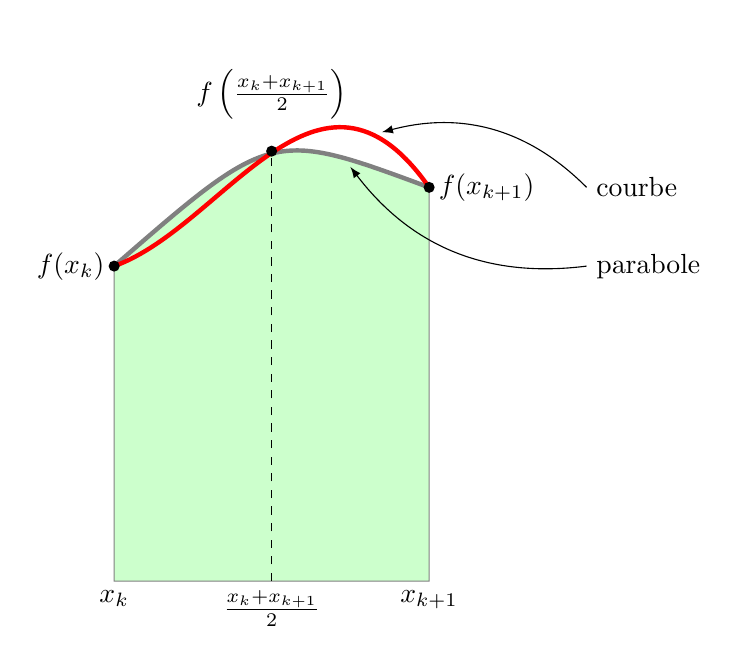
\begin{tikzpicture}[scale=2]

% Simpson

\filldraw[fill=green!20,draw=gray] (1,0)--(1,2) .. controls (2,2.87)..(3,2.5)--(3,0)--cycle;

\draw[ultra thick, color=gray] (1,2) .. controls (2,2.87)..(3,2.5);

\draw[ultra thick, color=red] (1,2).. controls (1.7,2.25) and (2.3,3.5) ..  (3,2.5);

\draw[dashed] (2,0)--(2,2.73);
  \fill (2,2.73) circle (1pt) node[above=8pt] {$f\left(\frac{x_k+x_{k+1}}{2}\right)$};
 \node[below] at (1,0) {$x_k$};
 \node[below] at (2,0) {$\frac{x_k+x_{k+1}}{2}$};
 \node[below] at (3,0) {$x_{k+1}$};
 \fill (1,2) circle (1pt) node[left]  {$f(x_k)$};
 \fill(3,2.5)  circle (1pt)node[right] {$f(x_{k+1})$};


   \draw[<-,>=latex] (2.7,2.85)to[bend left] (4,2.5)  node[right]{courbe};
   \draw[<-,>=latex] (2.5,2.63)to[bend right] (4,2)  node[right]{parabole};
\end{tikzpicture}

} 
%Cette parabole est la parabole passant par les trois
%points de la courbe  : 
%\begin{itemize}
%  \item $\big( \alpha, f(\alpha) \big)$,
%  \item $\big( \beta, f(\beta) \big)$,
%  \item et le point dont l'abscisse est le milieu :
%$\big( \frac{\alpha+\beta}{2}, f\left( \frac{\alpha+\beta}{2}\right)\big)$.
%\end{itemize}
%
%Il se trouve que l'aire sous cette portion de parabole se calcule très facilement,
%c'est :
%$$\frac{\beta-\alpha}{6} \left( f(\alpha)+f(\beta) + 4f\left(\frac{\alpha+\beta}{2}\right) \right).$$ 
\end{itemize}  


\end{cours}


%%%%%%%%%%%%%%%%%%%%%%%%%%%%%%%%%%%%%%%%%%%%%%%%%%%%%%%%%%%%%%%%
% Activité 2
%%%%%%%%%%%%%%%%%%%%%%%%%%%%%%%%%%%%%%%%%%%%%%%%%%%%%%%%%%%%%%%%

\begin{activite}[Calcul approché d'intégrales]

\objectifs{Objectifs : programmer la méthode des rectangles, des trapèzes et de Simpson.}

$$I = \int_a^b f(t) \;\dd t$$

\begin{enumerate}
  \item \textbf{Méthode des rectangles (à gauche).}
  
  \'Ecris une fonction \ci{integrale_rectangles(f,a,b,n)} qui renvoie une valeur approchée de l'intégrale $I$ par la formule :
  
  \mybox{$\displaystyle S_R(n) = \frac{b-a}{n}\sum_{k=0}^{n-1} f(x_k)$}
  
  \emph{Application.} Calcule une valeur approchée de $I_1 = \int_{1}^{2} \frac 1t \; \dd t$. Compare avec la valeur exacte (obtenue par primitive). \`A partir de quelle valeur de $n$ obtiens-tu $3$ chiffres exacts après la virgule ? Et pour obtenir $10$ chiffres exacts ?
  
    
  \item  \textbf{Méthode des trapèzes.}
  
  \'Ecris une fonction \ci{integrale_trapezes(f,a,b,n)} qui renvoie une valeur approchée de l'intégrale $I$ par la formule :
  \mybox{$\displaystyle S_T(n) = \frac{b-a}{n}\sum_{k=0}^{n-1} \frac{f(x_k)+f(x_{k+1})}{2}$}

  \begin{itemize}
  \item \emph{Application.} Recommence le calcul de $I_1 = \int_{1}^{2} \frac 1t \; \dd t$. Cherche quelles valeurs de $n$ permettent d'avoir $3$ chiffres exacts après la virgule, puis $10$ chiffres.
  
  \item 
  \begin{minipage}[t]{0.60\textwidth}   
  \emph{Application.} Fais le même travail pour calculer une valeur approchée de l'aire d'un disque de rayon $1$ par la formule $I_2 = 4 \int_0^1 \sqrt{1-t^2}\dd t$. 
  \end{minipage}\qquad
  \begin{minipage}[]{0.25\textwidth}      
\myfigure{0.5}{
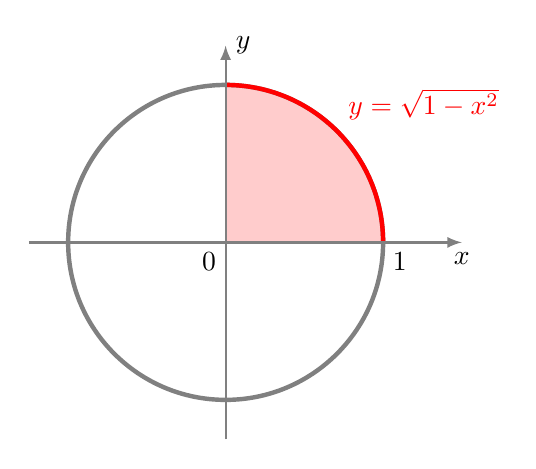
\begin{tikzpicture}[scale=1]

% Axes


  \fill[ultra thick, color=red!20] (0,0) -- (2,0)  arc (0:90:2cm) -- cycle;
    \draw[ultra thick, gray] (0,0) circle (2cm);
  \draw[ultra thick, color=red] (2,0) arc (0:90:2cm) node[midway,above right] {$y = \sqrt{1-x^ 2}$};

     \draw[->,>=latex,thick, gray] (-2.5,0)--(3,0) node[below,black] {$x$};
     \draw[->,>=latex,thick, gray] (0,-2.5)--(0,2.5) node[right,black] {$y$};  



  \node[below left] at (0,0) {$0$};
  \node[below right] at (2,0) {$1$};
%  \draw[blue, thick] (0,0)--(0,1) node[midway, left] {$1$};

\end{tikzpicture}
}    
 \end{minipage} 
  
   
  \end{itemize}
  
   
  \item  \textbf{Méthode de Simpson.}  
  
  \'Ecris une fonction \ci{integrale_simpson(f,a,b,n)} qui renvoie une valeur approchée de l'intégrale $I$ par la formule :
  \mybox{$\displaystyle S_S(n) = \frac{b-a}{n}\sum_{k=0}^{n-1} \frac{f(x_k)+4f(\frac{x_k+x_{k+1}}{2}) + f(x_{k+1})}{6}$}
  
  \begin{itemize}
  \item \emph{Application.} Recommence le calcul de $I_1 = \int_{1}^{2} \frac 1t \; \dd t$ et trouve les valeurs de $n$ qui permettent d'avoir $3$ chiffres exacts après la virgule, puis $10$ chiffres.
  
  \item \emph{Application.} Fais le même travail pour $I_2 = 4 \int_0^1 \sqrt{1-t^2} \; \dd t$.
   
  \item \emph{Application.} Trouve une valeur approchée de $I_3 = 4\int_0^1 \frac{1}{1+t^2} \; \dd t$. 
  \end{itemize}  
  
  \item \textbf{Bonus.}
  \begin{enumerate}
  
    \item     
    \begin{minipage}[t]{0.6\textwidth}    
   Programme une fonction qui calcule une valeur approchée d'une intégrale par la méthode des rectangles à droite : c'est-à-dire que sur l'intervalle $[x_k,x_{k+1}]$ on approche l'intégrale par le rectangle de hauteur $f(x_{k+1})$ (et pas celui de hauteur $f(x_k)$). 
   \end{minipage}
   \begin{minipage}[c]{0.25\textwidth}      
	\myfigure{0.5}{
	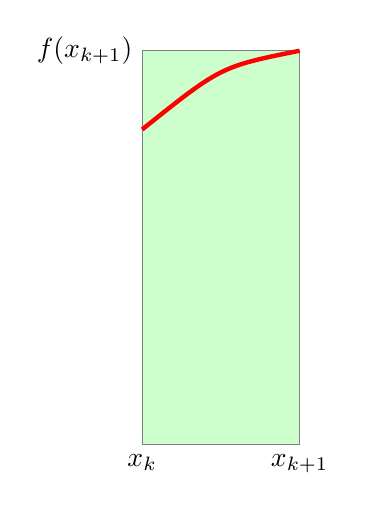
\begin{tikzpicture}[scale=2]



% Rectangle a droite (en vert)

\filldraw[fill=green!20,draw=gray] (1,0) rectangle (2,2.5);

  \draw[ultra thick, color=red] (1,2).. controls (1.5,2.4) ..  (2,2.5);

 \node[below] at (1,0) {$x_k$};
 \node[below] at (2,0) {$x_{k+1}$};
\node[left] at (1,2.5) {$f(x_{k+1})$};


\end{tikzpicture}
	}  
	\end{minipage}

  \item Montre que dans le cas d'une fonction monotone (croissante ou bien décroissante) les deux méthodes des rectangles (droite et gauche) fournissent un encadrement de l'intégrale. Déduis-en des encadrement des intégrales $I_1$, $I_2$, $I_3$.
  
  
  
 \item Pour la méthode des trapèzes, essaie d'écrire ta fonction de sorte qu'elle ne calcule  qu'une seule fois chaque $f(x_k)$.
 
 \item \emph{Projet.} Réalise la visualisation graphique des différentes méthodes.
  \end{enumerate} 
\end{enumerate} 

\end{activite}



%%%%%%%%%%%%%%%%%%%%%%%%%%%%%%%%%%%%%%%%%%%%%%%%%%%%%%%%%%%%%%%%
% Activité 3
%%%%%%%%%%%%%%%%%%%%%%%%%%%%%%%%%%%%%%%%%%%%%%%%%%%%%%%%%%%%%%%%



\begin{activite}[Intégrale de Gauss]

\objectifs{Objectifs : calculer une valeur approchée de l'intégrale de Gauss.}

On note 
$$I = \int_{-\infty}^{+\infty} e^{-t^2}\;\dd t \qquad
\text{ et } \qquad I(x) =  \int_{-\infty}^{x} e^{-t^2}\;\dd t.$$

\myfigure{0.6}{
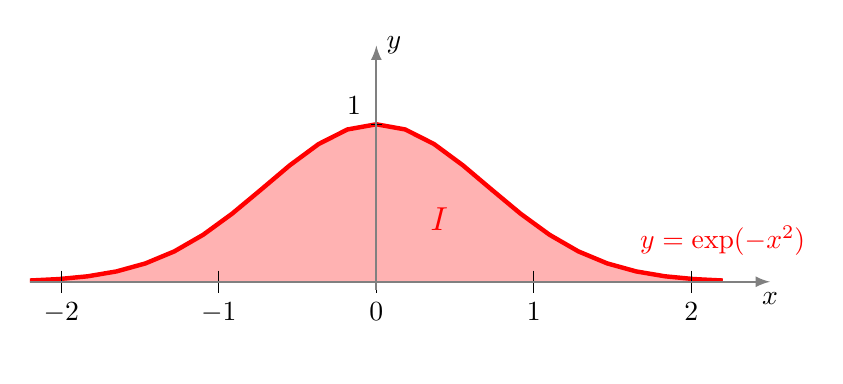
\begin{tikzpicture}[scale=2]

% Graphe et aire
  \fill[red!30] (-2.2,0) -- plot[domain=-2:2.2] (\x,{exp(-\x*\x)}) -- (2.2,0) -- cycle; 
% \node at (0.5,0.3) {$\mathcal{A}$};

%  \draw[gray] (-2,0) -- plot[domain=--2:2] (\x,{exp(-\x*\x)}) -- (2,0) -- cycle;
  \draw[ultra thick, color=red,domain=-2.2:2.2] plot (\x,{exp(-\x*\x)}) node[above=5pt] {$y=\exp(-x^2)$};

% Labels
  \foreach \x/\xtext in {-2/-2,-1/-1,0/0, 1/1, 2/2}
  \draw (\x cm,2pt) -- (\x cm,-2pt) node[anchor=north] {$\xtext$};
  \draw (1pt,1cm) -- (-1pt,1cm) node[anchor=south east] {$1$};
  \node[below, inner sep=10pt] at (0.5,0) {\vphantom{$n=10$}};

% Axes
     \draw[->,>=latex,thick, gray] (-2.2,0)--(2.5,0) node[below,black] {$x$};
     \draw[->,>=latex,thick, gray] (0,-0.05)--(0,1.5) node[right,black] {$y$};  

  \node[red,scale=1.2] at (0.4,0.4) {$I$};

\end{tikzpicture}
\qquad
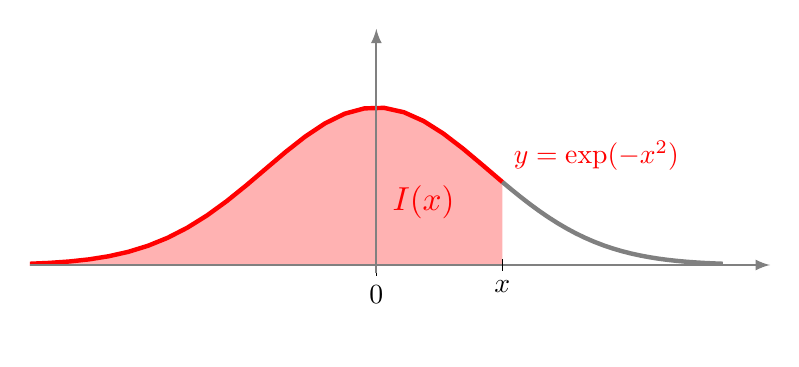
\begin{tikzpicture}[scale=2]

\def\A{0.8}
% Graphe et aire
  \fill[red!30] (-2,0) -- plot[domain=-2:\A] (\x,{exp(-\x*\x)}) -- (\A,0) -- cycle; 
% \node at (0.5,0.3) {$\mathcal{A}$};

  \draw[gray, ultra thick] plot[domain=\A:2.2] (\x,{exp(-\x*\x)}) ;
  \draw[ultra thick, color=red,domain=-2.2:\A] plot (\x,{exp(-\x*\x)}) node[above right] {$y=\exp(-x^2)$};

% Labels
  \foreach \x/\xtext in {0/0} %, 1/1, 2/2}
  \draw (\x cm,2pt) -- (\x cm,-2pt) node[anchor=north] {$\xtext$};
%  \draw (1pt,1cm) -- (-1pt,1cm) node[anchor=south east] {$1$};
  \node[below, inner sep=10pt] at (0.5,0) {\vphantom{$n=10$}};

% Axes
     \draw[->,>=latex,thick, gray] (-2.2,0)--(2.5,0) ; %node[below,black] {$x$};
     \draw[->,>=latex,thick, gray] (0,-0.05)--(0,1.5);  %node[right,black] {$y$};  

  \draw (\A cm,1pt) -- (\A cm,-1 pt) node[below] {$x$};

  \node[red,scale=1.2] at (\A-0.5,0.4) {$I(x)$};
\end{tikzpicture}

} 


Dans les exemples précédents, les intégrales à calculer avaient une valeur bien connue. C'est aussi le cas de l'intégrale de Gauss $I$ qui vaut $I = \sqrt\pi$. 
Par contre, en général, on ne saura pas calculer la valeur exacte d'une intégrale :
c'est le cas des intégrales $I(x)$. D'où l'intérêt d'en trouver des valeurs approchées.
\begin{enumerate}
  \item Programme une fonction \ci{integrale_gauss1()} qui renvoie une valeur approchée de $I$ et compare ta valeur avec $\sqrt \pi$.
  
  \emph{Indication.} Définis une grande valeur pour l'infini, par exemple en posant $N = 25$. Au lieu de calculer $\int_{-\infty}^{+\infty} f(t)\;\dd t$, tu calcules $\int_{-N}^{+N} f(t)\;\dd t$  (pour $|x|\ge 25$, $\exp(-x^2)$ est presque nul).
  
  \item Programme une fonction \ci{integrale_gauss2(x)} qui renvoie une valeur approchée de $I(x)$.
  
  \item Pour les calculs de probabilités, nous aurons besoin de calculer la loi normale dont la fonction de répartition est donnée par 
  $$I_{\mu,\sigma^2}(x) =  \frac{1}{\sqrt{2\pi\sigma^2}}\int_{-\infty}^{x} e^{-\frac{(t-\mu)^2}{\sigma^2}}\;\dd t$$ 
  où $\mu$ est l'espérance et $\sigma^2$ la variance ($\sigma$ est l'écart-type).
  
  Programme une fonction \ci{integrale_gauss3(x,mu,sigma2)} qui renvoie $I_{\mu,\sigma^2}(x)$.
  
  \item On modélise la répartition des personnes selon leur QI par une courbe de Gauss
  de paramètre $\mu = 100$ (le QI moyen) et $\sigma^2 = 225$ (écart-type $\sigma=15$). Avec ces paramètres $I_{\mu,\sigma^2}(x)$ représente le pourcentage de personnes ayant un QI inférieur à $x$. Par exemple $I(100) = 0.5$, donc $50\%$ de la population a un QI inférieur à $100$. Quel pourcentage de la population a un QI supérieur à $115$ ?
  
  
\myfigure{1.5}{
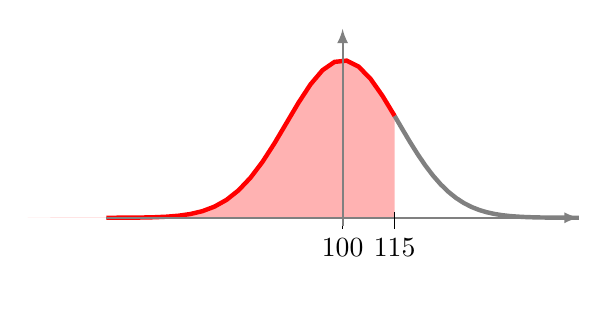
\begin{tikzpicture}[scale=2]

\def\A{0.33}
% Graphe et aire
  \fill[red!30] (-2,0) -- plot[domain=-1.5:\A] (\x,{exp(-4*\x*\x)}) -- (\A,0) -- cycle; 
% \node at (0.5,0.3) {$\mathcal{A}$};

  \draw[gray, ultra thick] plot[domain=\A:1.5] (\x,{exp(-4*\x*\x)}) ;
  \draw[ultra thick, color=red,domain=-1.5:\A] plot (\x,{exp(-4*\x*\x)}); % node[above right] {$y=\exp(-x^2)$};

% Labels
  \foreach \x/\xtext in {0/100} %, 1/1, 2/2}
  \draw (\x cm,2pt) -- (\x cm,-2pt) node[anchor=north] {$\xtext$};
%  \draw (1pt,1cm) -- (-1pt,1cm) node[anchor=south east] {$1$};
  \node[below, inner sep=10pt] at (0.5,0) {\vphantom{$n=10$}};

% Axes
     \draw[->,>=latex,thick, gray] (-1.5,0)--(1.5,0) ; %node[below,black] {$x$};
     \draw[->,>=latex,thick, gray] (0,-0.05)--(0,1.2);  %node[right,black] {$y$};  

  \draw (\A cm,1pt) -- (\A cm,-2 pt) node[below] {$115$};

 % \node[red,scale=1.2] at (\A-0.5,0.4) {$I(x)$};
\end{tikzpicture}

}    
  
\end{enumerate} 

\end{activite}



\end{document}
